\documentclass{article}

\usepackage{amsmath}
\usepackage{amssymb}
\usepackage{amsfonts}
\usepackage{mathtools}

\usepackage[thmmarks, amsmath]{ntheorem}

\usepackage{graphicx}

\usepackage{diffcoeff}
\diffdef{}{op-symbol=\mathrm{d},op-order-sep=0mu}

\usepackage{cancel}

\usepackage{enumitem}

\setlist{label=\alph*)}

\title{Proof of Corollary 3}
\author{Duarte Maia}
%\date{}

\theorembodyfont{\upshape}
\theoremseparator{.}
\newtheorem{theorem}{Theorem}
\newtheorem{prop}{Prop}
\renewtheorem*{prop*}{Prop}
\newtheorem{lemma}{Lemma}

\theoremstyle{nonumberplain}
\theoremheaderfont{\itshape}
\theorembodyfont{\upshape}
\theoremseparator{:}
\theoremsymbol{\ensuremath{\blacksquare}}
\newtheorem{proof}{Proof}

\newcommand{\R}{\mathbb{R}}
\newcommand{\C}{\mathbb{C}}

\newcommand{\PP}{\mathbb{P}}
\newcommand{\FF}{\mathcal{F}}

\newcommand{\I}{\mathrm{i}}
\newcommand{\e}{\mathrm{e}}


\DeclareMathOperator{\inte}{int}
\DeclareMathOperator{\codim}{codim}
\newcommand{\grad}{\nabla}

\DeclarePairedDelimiter{\norm}{\lvert}{\rvert}
\DeclarePairedDelimiter{\Norm}{\lVert}{\rVert}

\newcommand{\corthree}{Corollary 3}

\begin{document}
\maketitle

\section{Introduction}

In this document I prove the following statement, which is useful for a construction of good covers which does not use tools from Riemannian Geometry.

\begin{prop*}[\corthree]
Let $U$ and $V$ be neighborhoods of the origin in $\R^n$, and $f \colon U \to V$ a diffeomorphism. Suppose also that $f(0) = 0$ and $\dl f(0) = I$. Then, for all small enough $r > 0$, $f(B_r(0))$ is convex.
\end{prop*}

This statement would not be true if instead of balls we were considering cubes, so why should we expect it to be true for balls? Well, the idea is that the convexity of a cube is a fragile thing, because its surface is straight, but since a ball is curved inward you require large enough deformations to overcome the curvature.

This intuitive argument makes recourse to curvature, a $C^2$ property, so it slightly hints that the proof might require $C^2$ diffeomorphisms. Indeed, the proof outlined below does (or at the very least that the derivative be loc. Lipschitz), but I do not know whether a $C^1$ counterexample exists.

\section{Pre-Proof}

In order to prove \corthree, we will reduce it to a much simpler problem.

Indeed, statements of convexity are, in some sense, global, but the tools we have to work with (derivatives) are local in nature. To this effect, we will reduce the issue to a local problem.

We begin by asking the question: What must happen for $f(B_r(0))$ not to be convex? Well, there must exist $x, y \in B_r(0)$ such that the line segment connecting $f(x)$ and $f(y)$ is not entirely contained in $f(B_r(0))$. In other words, some point of the form
\[u = t_0 f(x) + (1-t_0) f(y)\]
is not in $f(B_r(0))$.

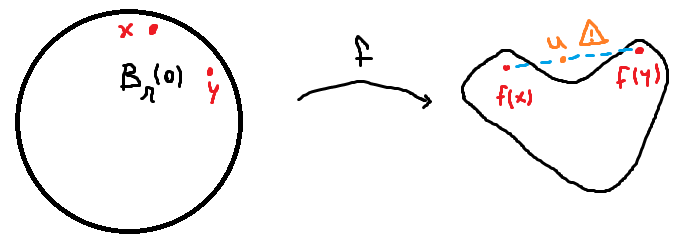
\includegraphics[width=\linewidth]{c3i1}

The first simplification we will do is the following: We will shrink the line segment around $u$ as much as possible, so that $f(x)$ and $f(y)$ lie just inside the ball, and that the line segment connecting them immediately leaves the ball. This shrinkage might not be possible (or rather, might be trivial) if $u$ lies just outside the ball, so we will change our goal slightly, proving instead that the image of the \emph{closed} ball is convex. In other words, we will prove that a scenario such as below cannot happen (for small enough $r$).

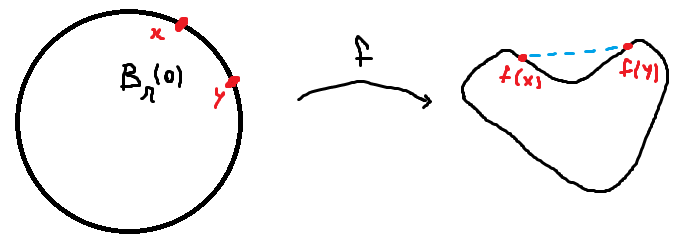
\includegraphics[width=\linewidth]{c3i2}

This is a much easier requirement, because we can obtain a contradiction via derivatives at $x$ or $y$. Indeed, let $\gamma(t)$, $t \in [0,1]$ be the blue curve, starting at $x$ and ending at $y$. If we were to show that $\dot\gamma(0)$ points inwards into the ball, we would immediately obtain a contradiction. Therefore, in the next section we prove the following lemma:

\begin{lemma}\label{gointoball}
Let $U$, $V$ and $f$ be in the hypotheses of \corthree. Then, for small enough $r$, the following is true.

Let $x, y \in \partial B_r(0)$ be two distinct points, and set $\gamma(t) = (1-t) f(x) + t f(y)$. Define $\eta(t) = f^{-1}(\gamma(t))$, which is defined for small enough $t$. Then, $\dot \eta(0)$ points inwards into the ball, i.e. $x \cdot \dot \eta(0) < 0$.
\end{lemma}

We now outline the proof of \corthree from this lemma. All following propositions assume $U$, $V$ and $f$ in the hypotheses of \corthree.

\begin{prop}
For small enough $r$, $f(\overline{B_r(0)})$ is convex.
\end{prop}

\begin{proof}
By small enough $r$, we mean $r$ small enough for lemma \ref{gointoball} to apply.

Suppose that $r$ is small enough and that $f(\overline{B_r(0)})$ is not convex. Then, there must exist $x_0$ and $y_0$, with norm in $[0,r]$, and $t_0 \in \left]0,1\right[$, such that $\gamma_0(t) \not \in f(\overline{B_r(0)})$, where
\[\gamma_0(t) = (1-t) f(x_0) + t f(y_0).\]

Now, consider $A = \gamma_0^{-1}(f(\partial B_r(0)))$. This is a closed set, which clearly does not contain $t_0$, but contains $0$ and $1$. Therefore, there must exist a maximal element of $A$ which is less than $t_0$, say $t_-$, and a minimal element of $A$ which is greater than $t_0$, say $t_+$.

The idea is that $f^{-1}(\gamma_0(t_\pm))$ are the $x$ and $y$ to which we apply the previous lemma, as they are both in the border of $B_r(0)$ and the line segment which connects them is entirely outside of $\overline{B_r(0)}$ (this is a trivial application of Bolzano's theorem to $R \circ \gamma_0$, where $R$ is the pushforward of the norm via $f$).

Indeed, consider this pair $x$,$y$. These two points are clearly distinct, because there is a point in the line segment connecting them which is outside of the circle. We may then define $\gamma$ and $\eta$ as in the statement of lemma \ref{gointoball}, and this lemma tells us that
\[x \cdot \eta(t) < 0.\]

On the one hand, we know by minimality and maximality of $t_\pm$ that every point in $\gamma$ except the extrema is not in $f(\overline{B_r(0)})$. In other words, $\norm{\eta(t)}^2 > r^2$ for $t \neq 0, 1$. On the other hand,
\[\diff{\norm{\eta(t)}^2}t[0] = 2 \eta(0) \cdot \dot\eta(0) = 2 x \cdot \dot\eta(0) < 0,\]
which implies that $\norm{\eta(t)}^2 < \norm{\eta(0)}^2 = r^2$ for small enough positive $t$, which is a clear contradiction.

This shows that our initial hypothesis (that $f(\overline{B_r(0)})$ was not convex) is false, and this concludes the proof.
\end{proof}

\begin{prop}[\corthree]
For small enough $r$, $f(B_r(0))$ is convex.
\end{prop}

\begin{proof}
Notice that $f(B_r(0)) = \bigcup_{\rho<r} f(\overline{B_\rho(0)})$, and that increasing unions of convex sets are convex.
\end{proof}

\section{Proof of Lemma \ref{gointoball}}

We recall the hypotheses of the lemma:

Let $U$ and $V$ be neighborhoods of the origin, and $f \colon U \to V$ a diffeomorphism. Let $r$ be small enough (we will give a precise bound later), and let $x, y \in \partial B_r(0)$ be two distinct points. Define the two curves
\[\gamma(t) = (1-t) f(x) + t f(t), \; \eta(t) = f^{-1}(\gamma(t)).\]
Note that $\eta$ is defined for all $t \in [0,1]$ if $r$ is small enough.

We will show that $x \cdot \dot \eta(0) < 0$. To this effect, we begin by calculating this term explicitly:
\[x \cdot \dot \eta(0) = x \cdot (\dl f^{-1})_{f(x)} (\dot \gamma(0)) ) = x \cdot (\dl f)_x^{-1} (f(y) - f(x)).\]

Rougly speaking, the idea is that $\dl f$ is close to $I$ and that $f(y)-f(x)$ is close to $x-y$, so that we get
\[x \cdot \dot \eta(0) \approx x \cdot (y-x) = x \cdot y - x \cdot x \leq \norm x \norm y - \norm x ^2 = r^2 - r^2 = 0,\]
with equality if and only if we have equality in the Cauchy-Schwarz step, i.e. if $x$ and $y$ are colinear (with a positive constant), which, since they both have the same norm, happens iff $x=y$ , which is false by hypothesis.

Unfortunately, the estimates required are subtle, so we will tread with care.

The following argument is inspired by the proof of the Taylor series theorem for $\R^n$. We begin with a triviality:
\begin{multline*}
(\dl f)_x^{-1} (f(y)-f(x)) = \int_0^1 (\dl f)_x^{-1} \diff*{f((1-t) x + t y)}t \dl t\\
= \int_0^1 (\dl f)_x^{-1} (\dl f)_{tx + (1-t)y} (y-x) \dl t = \left( \int_0^1 (\dl f)_x^{-1} (\dl f)_{tx + (1-t)y} \dl t \right) (y-x).
\end{multline*}

Now we ask the question: How far can $(\dl f)_x^{-1} (\dl f)_{tx + (1-t)y}$ be from being the identity? Here is where we require a $C^2$ assumption on $f$, because we may use the second derivative to bound the operator distance between this expression and the identity. Indeed, we will show that (by decreasing $U$ and $V$ slightly if necessary, which poses no problem given that our proposition is only for small radii) there exists a constant $M$ such that
\begin{equation}\label{opnorm}
\Norm{(\dl f)_x^{-1} (\dl f)_{z} - I} \leq M \norm{x-z}.
\end{equation}

The proof of \eqref{opnorm} is outlined below, see lemma \ref{opnormlemma}

Taking \eqref{opnorm} for granted for the time being, we continue the proof. By the triangle inequality for integrals,
\begin{align*}
\norm*{\int_0^1 (\dl f)_x^{-1} (\dl f)_{tx + (1-t)y} (y-x) \dl t} &\leq
\int_0^1 \Norm{(\dl f)_x^{-1} (\dl f)_{tx + (1-t)y} - I} \dl t\; \norm{x-y}\\
&\leq M \norm{x-y}^2.
\end{align*}

As a consequence, $x \cdot \dot\eta(0)$ differs from $x \cdot (y-x)$ by a factor of at most $M r \norm{x-y}^2$. (The extra $r$ term comes from the inner product with $x$, which has norm $r$, and Cauchy-Schwarz.)

We may now consider `small enough' to mean $r < \frac1{2M}$, whence we get
\begin{align*}
x \cdot \dot\eta(0) &< x \cdot (y-x) + \frac12 \norm{x-y}^2\\
&= \left( x + \frac12 (y-x) \right) \cdot (y-x)\\
&= \frac12 (y+x) \cdot (y-x)\\
&= \frac12 (\norm{y}^2 - \norm{x}^2) = \frac12(r^2 - r^2) = 0.
\end{align*}

The proof of lemma \ref{gointoball} is now complete, and with it the proof of \corthree, modulo the following lemma:


\begin{lemma}\label{opnormlemma}
Suppose that we shrink $U$ a little bit, in order to ensure that all continuous quantities defined on $U$ are now bounded. Then, there exists a constant $M$ such that, for $x$ and $z$ in (the new, shrunk) $U$,
\[\Norm{(\dl f)_x^{-1} (\dl f)_{z} - I} \leq M \norm{x-z}.\]
\end{lemma}

\begin{proof}
The first step is to note that, by continuity of the operator norm, the expression $\Norm{(\dl f)_x}$ is bounded from above and below, and consequently there exists $M_1$ such that $\frac1{\Norm{(\dl f)_x}} \leq M_1$ for all $x \in U$.

Next, by the rule of composition of operator norm, it is easy to conclude
\[\Norm{(\dl f)_x^{-1} (\dl f)_{z} - I} \leq \frac1{\Norm{(\dl f)_x}} \Norm{(\dl f)_{z} - (\dl f)_x} \leq M_1 \Norm{(\dl f)_{z} - (\dl f)_x},\]
so now it suffices to find a bound for $\Norm{(\dl f)_{z} - (\dl f)_x}$.

To this effect, will use the second derivative to find a bound for the infinity norm of the matrix $A(z,x) := (\dl f)_{z} - (\dl f)_x$. The infinity norm of a matrix is the maximum absolute value of its entries. It is easy to show
\[\Norm{(\dl f)_{z} - (\dl f)_x} \leq n^2 \Norm{(\dl f)_{z} - (\dl f)_x}_\infty,\]
and to bound the infinity norm of a matrix we look at its entries, which are in this case
\[A(z,x)_{ij} = \partial_j f^i(z) - \partial_j f^i(x).\]

An easy application of Lagrange's theorem will show that
\[A(z,x)_{ij} = \sum_k \partial_k \partial_j f^i(\xi) (z-x)_i\]
for some $\xi$ depending on (and in between) $z$ and $x$, whence
\[\norm{A(z,x)_{ij}} \leq n M_2 \norm{z-x},\]
where $M_2$ is a bound for all second derivatives of $f$ on $U$.

The lemma has now been shown, for $M = n^3 M_1 M_2$. 
\end{proof}

\end{document}